\documentclass{article}
\usepackage[slovene]{babel}
\usepackage[utf8]{inputenc}
\usepackage[T1]{fontenc}
\usepackage{amsmath, amssymb}
\usepackage{amsthm}
\usepackage{graphicx}
\usepackage{comment}
\usepackage{caption}

\newcommand{\program}{Finančna matematika} % ime studijskega programa: Matematika/Finančna matematika
\newcommand{\imeavtorja}{Oskar Težak, Sara Šega} % ime avtorja
\newcommand{\imementorja}{doc. dr. Janoš Vidali} % akademski naziv in ime mentorja
\newcommand{\imesomentorja}{prof. dr. Riste Škrekovski}
\newcommand{\naslovdela}{Laplacian integral graphs}
\newcommand{\letnica}{2024} %letnica 


\begin{document}

%naslovnica

\thispagestyle{empty}
\noindent{\large
UNIVERZA V LJUBLJANI\\[1mm]
FAKULTETA ZA MATEMATIKO IN FIZIKO\\[5mm]
\program\ }
\vfill

\begin{center}{\large
\imeavtorja\\[2mm]
{\bf \naslovdela}\\[10mm]
Skupinski projekt\\[2mm]
Poročilo\\[1cm]
Mentorja: \imementorja, \\ \imesomentorja\\[2mm]}
\end{center}
\vfill

\noindent{\large
Ljubljana, december \letnica}
\pagebreak




\section{Opis problema}

Poiskati želimo čim več enocikličnih in dvocikličnih grafov, katerih Laplaceove lastne vrednosti so cela števila. 
Za grafe nižjega reda to storimo z izčrpno metodo, za grafe višjega reda moramo uporabiti stohastično metodo. 
Najti želimo metodo oz. vzorec za generiranje Laplaceovih celoštevilskih grafov. \\ 
Naj bo $G(V,E)$ graf z množico vozlišč $V$, $ \left| V \right| = n $
in množico povezav $E$, $\left| E \right| = m. $ \\
Definiramo Laplaceovo matriko $ L = D - A $, kjer je $D$ $ n \times n $ diagonalna matrika, katere diagonalni členi so stopnje vozlišč grafa $G$, 
$A$ pa je $ n \times n $ matrika sosednosti. Elementi Laplaceove matrike $L$ so torej

\[
l_{i,j} = 
\begin{cases} 
    \deg(v_i), & \text{če } i = j, \\
    -1, & \text{če } i \neq j \text{ in } v_i \text{ je soseden z } v_j, \\
    0, & \text{sicer}.
\end{cases}
\]

Lastne vrednosti matrike $L$ so $ \lambda_1 \leq \lambda_2 \leq \dots \leq \lambda_n .$ Če so vse lastne
vrednosti pozitivne, pravimo, da je graf $G$ z matriko $L$ Laplaceov celoštevilski. 


\begin{comment}


\section{Potek}

Najprej sva napisala kodo za generiranje enocikličnih grafov, ki imajo relativno malo vozlišč. Uporabila sva dejstvo, da imajo povezani enociklični grafi enako
število povezav in vozlišč. Implementirala sva funkcijo, ki za vsak graf potem preveri, če je Laplaceov in Laplaceove tudi izriše. Funkcijo sva testirala
na grafih s 6, 7, 8, 9, 10 vozlišči. Za iskanje dvocikličnih grafov sva uporabila isto kodo, le da sva tokrat nastavila, da generirava grafe z $n$ vozlišči in $n+1$ povezavami.    

\[
\det(L - \lambda I) = 
\begin{vmatrix}
    n-k - \lambda &-1  &-1 &&\dots&&   -1  \\
    -1 & 2 - \lambda & -1&&&&  &    \\
    -1&  -1 & \ddots &\ddots&&&  & \\
    &  &\ddots  & 2 - \lambda &&&&    \\
    \vdots& &  &  &1 - \lambda &&  & \\
    &  &  &  &  &\ddots \\
    -1& &  &  &  & &1 - \lambda \\
\end{vmatrix}
\]
\end{comment}
\section{Generiranje enocikličnih Laplaceovih celoštevilskih grafov}
Za generiranje povezanih enocikličnih grafov sva uporabila funkcijo $nauty$ $geng$ in dejstvo, da za povezane enociklične grafe velja, 
da je njihovo število vozlišč enako številu povezav. S funkcijo $ is\_laplacian\_integer\_graph(G) $ sva potem preverjala, kateri izmed 
enocikličnih grafov imajo celoštevilske Laplaceove lastne vrednosti. To sva uporabila na manjših grafih (do 10 vozlišč) in opazila, da so 
Laplaceovi tisti, ki imajo eno centralno vozlišče, ki je del cikla, vsa vozlišča, ki niso del cikla, pa so tudi povezana s tem centralnim vozliščem. 
V splošnem bi njihova Laplaceova matrika bila $L=$
\begin{bmatrix}
    n-k  &-1  &-1 &&\dots&&   -1  \\
    -1 & 2  & -1&&&&  &    \\
    -1&  -1 & \ddots &\ddots&&&  & \\
    &  &\ddots  & 2 &&&&    \\
    \vdots& &  &  &1  &&  & \\
    &  &  &  &  &\ddots \\
    -1& &  &  &  & &1 \\
\end{bmatrix}, \\
njihov graf pa bi izgledal takole:

\begin{figure}[htbp]
    \centering
    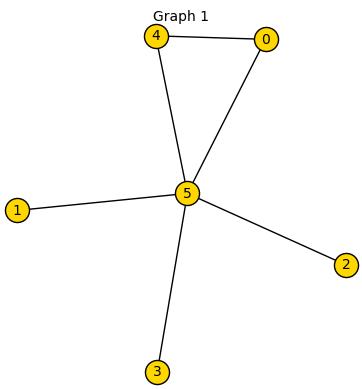
\includegraphics[width=0.5\textwidth]{primer_6.png}
    \caption{Celoštevilski Laplaceov graf s 6 vozlišči}
    \label{fig:izjema2}
\end{figure}

Izjema sta bila le grafa, ki sta imela vsa vozlišča vključena v cikel: \\
\begin{minipage}{0.5\textwidth}
    \centering
    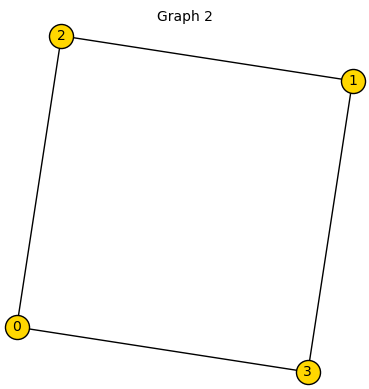
\includegraphics[width=0.7\textwidth]{izjema1.png}
    \captionof{figure}{Graf s 4 vozlišči}
\end{minipage}
\begin{minipage}{0.5\textwidth}
    \centering
    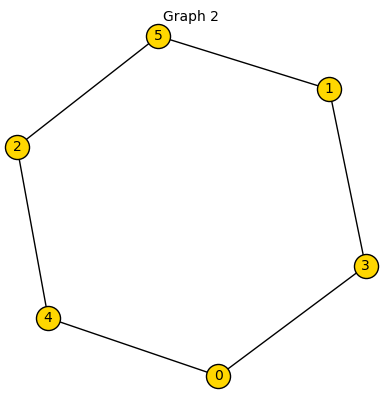
\includegraphics[width=0.7\textwidth]{izjema2.png}
    \captionof{figure}{Graf s 6 vozlišči}
\end{minipage}
\par
Opazko glede oblike sva želela preveriti v datoteki $shape\_hypotesis.ipynb$. Generirala sva enociklične grafe s centralnim vozliščem, in sicer tako, da sva v poljubnem ciklu 
izbrala centralno vozlišče, nato pa dodajala vozlišča, ki so bila vsa povezana s centralnim vozliščem. Za generirane grafe sva preverila celoštevilskost lastnih vrednosti in 
na podlagi najinih testiranj ugotovila, da hipoteza o takšni obliki velja le za enociklične grafe, ki imajo cikel dolžine 3. \\
Za iskanje enocikličnih Laplaceovih celoštevilskih grafov z večjim številom vozlišč sva uporabila stohastično metodo. Najprej sva napisala funkcijo,
ki generira enociklične grafe, nato pa sva s funkcijo $unicyclic\_laplacian\_integer\_graph\_stohastic$ preverila, kateri izmed njih so Laplaceovi celoštevilski. 
Funkcijo sva testirala tako, da sva za grafe z 10 do 100 vozlišči generirala največ 10000 enocikličnih grafov in za te preverila, koliko je celoštevilskih Laplaceovih.
Izkazalo se je, da ni bil nobeden.

\section{Generiranje dvocikličnih Laplaceovih celoštevilskih grafov}
Podobno kot pri enocikličnih grafih, sva tudi v tem primeru najprej ustvarila funkcijo, ki generira dvociklične grafe in jih potem testirala, če so celoštevilski 
Laplaceovi. To funkcijo sva uporabila na grafih z majhnim številom vozlišč. 

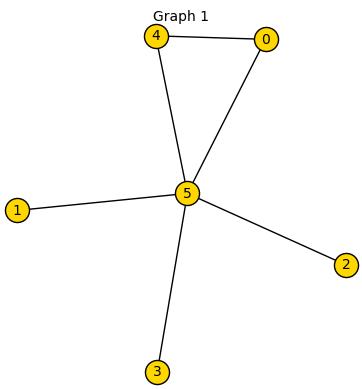
\includegraphics[width=0.5\textwidth]{primer_6.png} \\
Za večje grafe sva uporabila stohastično metodo, in sicer sva najprej generirala dvociklične grafe (ustvarimo
2 poljubna cikla in ju potem povežemo), potem pa preverjamo, ali imajo celoštevilske lastne vrednosti. Zopet se je po testiranju izkazalo, da so celoštevilski
Laplaceovi grafi redki, saj med dvocikličnimi grafi z 10 do 100 vozlišči, ni bilo nobenega.

\section{Generiranje grafov s čim več celoštevilskih lastnih vrednosti}

\end{document}